\section{Propriedades da probabilidade}

\begin{lemma}\label{lem:ch01-vazio}
    $\emptyset$ denota o evento impossível.

    Temos que $\Prob(\emptyset) = 0$.
\end{lemma}

\begin{proof}
    Seja $A \in \F$ tal que $\Prob(A) > 0$. Podemos escrever
    \begin{align*}
        A &= A \cup \left(\bigcup_{i=1}^\infty B_i\right),
    \end{align*}
    em que $B_i = \emptyset$. Note que $A$ e $B_i$ 
    são mutuamente exclusivos. Pelo axioma \labelcref{it:ch01-axioma-2} 
    da \cref{def:axiomatica}:
    \begin{align*}
        \Prob(A) &= \Prob(A) +
            \left(\sum_{i=1}^\infty \Prob(B_i)\right) \\
        &= \Prob(A) +
            \left(\sum_{i=1}^\infty \Prob(\emptyset)\right)
    \end{align*}
    de modo que
    \begin{align*}
        \sum_{i=1}^\infty \Prob(\emptyset) &= 0.
    \end{align*}
    Pelo axioma \labelcref{it:ch01-axioma-1} 
    da \cref{def:axiomatica}, $\Prob(\emptyset) \geq 0$.
    Portanto, $\Prob(\emptyset) = 0$.
\end{proof}

\begin{lemma}\label{lem:ch01-uniao-finita}
    Se os eventos $A_1, \cdots, A_n$ em $\F$ são mutuamente exclusivos,
    \begin{align}
        \Prob\left(\bigcup_{i=1}^n A_i\right) &=
            \sum_{i=1}^n \Prob(A_i) \label{eq:ch01-uniao-finita}
    \end{align}
\end{lemma}

\begin{proof}
    Seja $B_1, B_2, \cdots$ uma sequência de eventos disjuntos em $\F$,
    definidos por
    \begin{align*}
        B_i &= \begin{cases}
            A_i,&\ i = 1,\cdots,n \\
            \emptyset,&\ i = n + 1,\cdots
        \end{cases},
    \end{align*}
    de modo que
    \begin{align*}
        \bigcup_{i=1}^\infty B_i &= \bigcup_{i=1}^n A_i
    \end{align*}
    Pelo axioma \labelcref{it:ch01-axioma-1} da \cref{def:axiomatica}
    e recordando o \cref{lem:ch01-vazio}, temos que
    \begin{align*}
        \Prob\left(\bigcup_{i=1}^\infty B_i\right)
            &= \Prob\left(\bigcup_{i=1}^n A_i\right) \\
            &= \sum_{i=1}^\infty \Prob(B_i) \\
            &= \sum_{i=1}^n \Prob(B_i) + \sum_{i=n+1}^\infty \Prob(B_i) \\
            &= \sum_{i=1}^n \Prob(A_i)
            +  \sum_{i=n+1}^\infty \cancelto{0}{\Prob(\emptyset)} \\
            &= \sum_{i=1}^n \Prob(A_i)
    \end{align*}
    Portanto,
    \begin{align*}
        \Prob\left(\bigcup_{i=1}^n A_i\right) 
            &= \sum_{i=1}^n \Prob(A_i)
    \end{align*}
\end{proof}

\begin{lemma}\label{lem:ch01-complemento}
    Se $\stcomp{A}$ denota o complemento do evento $A$, então
    \begin{align}
        \Prob(\stcomp{A}) = 1 - \Prob(A) \label{eq:ch01-complemento}
    \end{align}

    \begin{obs}
        Se $A \in \F$, então $\stcomp{A} \in \F$.
    \end{obs}
\end{lemma}

\begin{proof}
    Recordamos que $A \cup \stcomp{A} = S$. Além disso,
    pelo axioma \labelcref{it:ch01-axioma-3} da \cref{def:axiomatica},
    $\Prob(S) = 1$. Com estas informações, e usando o \cref{lem:ch01-uniao-finita}, temos que:
    \begin{align*}
        A \cup \stcomp{A} &= S \\
        \implies \Prob(A \cup \stcomp{A}) &= \Prob(S) \\
        \implies \Prob(A) + \Prob(\stcomp{A}) &= \Prob(S) \\
        \implies \Prob(A) + \Prob(\stcomp{A}) &= 1 \\
        \therefore \Prob(\stcomp{A}) &= 1 - \Prob(A)
    \end{align*}
    Portanto,
    \begin{align*}
        \Prob(\stcomp{A}) &= 1 - \Prob(A)
    \end{align*}
\end{proof}

\begin{lemma}\label{lem:ch01-subconjunto}
    Se $A \in \F$, $B \in \F$ e $A \subset B$,
    então $\Prob(A) \leq \Prob(B)$
\end{lemma}

\begin{proof}
    Primeiro, note que $B = A \cup (\stcomp{A} \cap B)$.
    \begin{center}
        \begin{tikzpicture}
            \pgfmathsetmacro{\R}{0.5}
            \coordinate (A) at (-4, -2);
            \coordinate (C) at (4, 2);
            \coordinate (P) at (-2, 0);
            \coordinate (R) at (-2+\R, 0);

            \pgfmathsetmacro{\A}{3}
            \pgfmathsetmacro{\B}{1.5}
            \coordinate (Q) at (0, 0);
            \coordinate (S) at (\A, 0);
            
            \draw[ultra thick] (A) rectangle (C);
            \node[anchor=south east, ultra thick] at (C) {$S$};
            
            \draw[name path=inner, ultra thick] (P) circle (\R);
            \node[anchor=east, ultra thick] at (R) {$A$};

            \draw[name path=outer, ultra thick] (Q)
                ellipse [x radius=\A, y radius=\B];
            \node[anchor=west, ultra thick] at (S) {$B$};

            \tikzfillbetween[of=inner and outer, on layer=bg]
                {blue, opacity=0.2};
            \node[anchor=center, ultra thick, blue]
                at (Q) {$\stcomp{A} \cap B$};
        \end{tikzpicture}
    \end{center}
    Além disso, $A$ e $\stcomp{A} \cap B$ são eventos mutuamente exclusivos.
    Recordando o \cref{lem:ch01-uniao-finita}, temos:
    \begin{align*}
        \Prob(B) &= \Prob(A \cup (\stcomp{A} \cap B)) \\
            &= \Prob(A) + \Prob(\stcomp{A} \cap B) \\
        \implies \Prob(B) - \Prob(A) &= \Prob(\stcomp{A} \cap B) \\
    \end{align*}
    Pelo axioma \labelcref{it:ch01-axioma-1} da \cref{def:axiomatica},
    sabemos que $\Prob(\stcomp{A} \cap B) \geq 0$. Assim
    \begin{align*}
        \Prob(B) - \Prob(A) &= \Prob(\stcomp{A} \cap B) \geq 0 \\
        \implies \Prob(B) - \Prob(A) &\geq 0 \\
        \therefore \Prob(B) &\geq \Prob(A) \\
    \end{align*}
    Portanto,
    \begin{align*}
        \Prob(A) &\leq \Prob(B) \\
    \end{align*}
\end{proof}

\begin{lemma}\label{lem:ch01-uniao-dois}
    Se $A$ e $B$ são dois eventos de $\F$, então
    \begin{align}
        \Prob(A \cup B) = \Prob(A) + \Prob(B) - \Prob(A \cap B)
            \label{eq:ch01-uniao-dois}
    \end{align}
\end{lemma}

\begin{proof}
    Primeiro, note que:
    \begin{align*}
        A \cup B &= A \cup (\stcomp{A} \cap B)
    \end{align*}
    sendo que os eventos $A$ e $(\stcomp{A} \cap B)$ são mutuamente exclusivos; e
    \begin{align*}
        B &= (\stcomp{A} \cap B) \cup (A \cap B)
    \end{align*}
    em que $(\stcomp{A} \cap B)$ e $(A \cap B)$ são mutuamente exclusivos.
    Temos que
    \begin{align*}
        \Prob(A \cup B) &= \Prob(A \cup (\stcomp{A} \cap B)) \\
        \Prob(A \cup B) &= \Prob(A) + \Prob(\stcomp{A} \cap B)
    \end{align*}
    e
    \begin{align*}
        \Prob(B) &= \Prob((\stcomp{A} \cap B) \cup (A \cap B)) \\
        &= \Prob(\stcomp{A} \cap B) + \Prob(A \cap B) \\
        \implies \Prob(\stcomp{A} \cap B) 
        &= \Prob(B) - \Prob(A \cap B)
    \end{align*}
    Combinando os dois últimos resultados, temos que
    \begin{align*}
        \Prob(A \cup B) &= \Prob(A) + \Prob(\stcomp{A} \cap B) \\
        &= \Prob(A) + \Prob(B) - \Prob(A \cap B)
    \end{align*}
    Portanto,
    \begin{align*}
        \Prob(A \cup B)
            &= \Prob(A) + \Prob(B) - \Prob(A \cap B)
    \end{align*}
\end{proof}

\begin{lemma}\label{lem:ch01-uniao-gen}
    Sejam $A_1, \cdots, A_n$ eventos de $\F$. Temos:
    \begin{enumerate}
        \item \begin{align}
            \Prob\left(\bigcup_{i=1}^n A_i\right)
                = 1 - \Prob\left(\bigcap_{i=1}^n \stcomp{A_i}\right)
            \label{eq:ch01-uniao-gen-1}
        \end{align}
        \item \begin{align}
            \Prob\left(\bigcup_{i=1}^n A_i\right)
                &= \Prob(A_1) 
                + \Prob(\stcomp{A_1} \cap A_2)
                + \Prob(\stcomp{A_1} \cap \stcomp{A_2} \cap A_3) \\
                &\phantom{=}
                + \cdots
                + \Prob(\stcomp{A_1} \cap \stcomp{A_2} \cap \cdots \cap A_n)
            \label{eq:ch01-uniao-gen-2}
        \end{align}
        \item \begin{align}
            \Prob\left(\bigcup_{i=1}^n A_i\right)
                &\leq \Prob(A_1) + \Prob(A_2) + \cdots + \Prob(A_n)
                = \sum_{i=1}^n \Prob(A_i)
                \label{eq:ch01-uniao-gen-3}
        \end{align}
    \end{enumerate}
\end{lemma}

\begin{lemma}[Regra de adição e subtração]\label{lem:ch01-add-sub}
    Sejam $A_1, \cdots, A_n$ eventos de $\F$. Temos:
    \begin{align}
        \Prob\left(\bigcup_{i=1}^n A_i\right)
            &= \sum_{i=1}^n \Prob(A_i) \notag \\
            &\phantom{=}
            - \sum_{i=1}^n \sum_{j > 1} \Prob(A_i \cap A_j) \notag \\
            &\phantom{=}
            + \sum_{i=1}^n \sum_{j > 1} \sum_{k > j}
                \Prob(A_i \cap A_j \cap A_k)  \label{eq:ch01-add-sub} \\
            &\phantom{=}
            - \sum_{i=1}^n \sum_{j > 1} \sum_{k > j} \sum_{m > k}
                \Prob(A_i \cap A_j \cap A_k \cap A_m) \notag \\
            &\phantom{=} + \cdots \notag \\
            &\phantom{=}
            + (-1)^{n - 1} \Prob(A_1 \cap A_2 \cap \cdots \cap A_n) \notag
    \end{align}
\end{lemma}

\begin{example}[Problema dos aniversários]
    Em um grupo com $n$ pessoas $(n \geq 2)$, calcule a pobabilidade
    de que todas elas façam aniversáio em dias diferentes.
    
    \bigskip
    Considere que o ano tem 365 dias, e com iguais distribuições
    dos anivesários.
    O espaço amostral $S$ pode ser descrito como:
    \begin{align*}
        S = \{&(a_1, a_2, \cdots, a_n) : \\
        & a_j \in \{1, 2, \cdots, 365\}, \\
        & j = 1, 2, \cdots, n
        \}
    \end{align*}
    de modo que
    \begin{align*}
        N &= 365 \cdot 365 \cdot \ldots \cdot 365 \\
        &= 365^n,\ n \leq 365
    \end{align*}
    Denote o evento po $A$. o número de elementos de $A$ é
    \begin{align*}
        m &= 365 \cdot 364 \cdot \ldots \cdot (365 - (n - 1))
    \end{align*}
    Calculamos
    \begin{align*}
        \Prob(A) &= \frac{m}{N} \\
        &= \frac{365 \cdot 364 \cdot \ldots \cdot (365 - (n - 1))}
            {365 \cdot 365 \cdot \ldots \cdot 365} \\
        &= \frac{365 \cdot (365 - 1) \cdot \ldots \cdot (365 - (n - 1))}
            {365 \cdot 365 \cdot \ldots \cdot 365} \\
        &= \cancelto{1}{\frac{365}{365}} \cdot \frac{365 - 1}{365}  \cdot \frac{365 - 2}{365}
        \cdot \ldots \cdot \frac{365 - (n - 1)}{365} \\
        &= \left(1 - \frac{1}{365}\right)
        \cdot \left(1 - \frac{2}{365}\right)
        \cdot \ldots
        \cdot \left(1 - \frac{n - 1}{365}\right) \\
    \end{align*}
    O evento $\stcomp{A}$ representa a situação em que pelo menos
    duas pessoas têm aniversário no mesmo dia, sendo que
    \begin{align*}
        \Prob(\stcomp{A}) = 1- \Prob(A)
    \end{align*}
    \begin{center}
        \begin{tabular}{cc}
            \toprule
            $n$ & $\Prob(\stcomp{A})$ \\
            \midrule
            23 & 0.5073 \\
            40 & 0.8912 \\
            60 & 0.9941 \\
            \bottomrule
        \end{tabular}
    \end{center}
\end{example}

\begin{example}
    Considere a equação de $2^o$ grau
    \begin{align*}
        x^2 + 2bx + c &= 0
    \end{align*}
    sendo que $b \in \R$ e $c \in \R$.
    
    Os valores de $b$ e $c$ são escolhidos ao acaso.
    
    Calcule a probabilidade de que a equação tenha raízes reais.

    \bigskip
    O discriminante $\Delta$ é dado por
    \begin{align*}
        \Delta &= (2b)^2 - 4c \\
        &= 4b^2 - 4c \\
        &= 4(b^2 - c)
    \end{align*}
    Para que as raízes sejam reais, devemos ter $\Delta \geq 0$.
    Representando graficamente, temos:
    \begin{center}
        \begin{tikzpicture}[
            declare function = { f(\x) = \x^2; }
            ]
            \pgfmathsetmacro{\b}{.5}
            \begin{axis}[
                unbounded coords=jump,
                grid=none,
                axis x line=middle,
                axis y line=middle,
                xmin=-2.5, xmax=2.5,
                ymin=-1, ymax=2,
                xtick=\empty,
                ytick=\empty,
                extra x ticks={-\b,\b},
                extra x tick labels={$-B$, $B$},
                extra y ticks={-\b,\b},
                extra y tick labels={$-B$, $B$},
                xlabel={$b$},
                ylabel={$c$},
                y label style={anchor=south},
                x label style={anchor=west},
            ]
            
            \addplot[
                name path=delta,
                samples=100,
                domain=-1.4:1.4,
                ultra thick,
                blue
            ] {f(x)};
            \node[blue, anchor=north west] (N) at (1.4, 1.96)
                {$c = b^2$};
            \node[blue, below of=N] 
                {$(\Delta = 0)$};

            \addplot[name path=upper, mark=none, ultra thick,  red]
                coordinates {(-5, 5) (5, 5)};

            \addplot[name path=lower, mark=none, ultra thick,  red]
                coordinates {(-5, -5) (5, -5)};

            \addplot [fill=orange, fill opacity=0.15]
                fill between[of=delta and upper,soft clip={domain=-1.4:1.4}];

            \addplot [fill=black, fill opacity=0.15]
                fill between[of=lower and delta,soft clip={domain=-1.4:1.4}];

            \node[orange] at (-0.7, 1.75) {$\Delta > 0$};
            \node[black] at (-0.7, -0.75)  {$\Delta < 0$};
            
            \addplot[name path=b, mark=none, red, dashed, thick
            ] coordinates {(-\b, \b) (\b, \b)};

            \draw[dashed, red, thick] (-\b, -\b) rectangle (\b, \b);

            \addplot [pattern=north west lines, pattern color=red]
                fill between[of=delta and b,soft clip={domain=-\b:\b}];
            
            \end{axis}
            \label{fig:ch01-eq-segundo-grau}
        \end{tikzpicture}
    \end{center}

    Delimitamos um quadado com lado de comprimento $2B$ centrado na origem, cuja área é $4B^2$.
    
    A área hachurada na figura é igual a $\frac{4}{3}B^\frac{3}{2}$.
    Portanto, a pobabilidade do evento é igual a
    \begin{align*}
        1 - \frac{\frac{4}{3}B^\frac{3}{2}}{4B^2}
        &= 1 - \frac{1}{3\sqrt{B}}
    \end{align*}
    Se $B = 4$, a probabilidade é
    \begin{align*}
        1 - \frac{1}{3\sqrt{4}} &= 1 - \frac{1}{6} = \frac{5}{6}
    \end{align*}

    Tomando o limite (quando $B \to \infty$), a probabilidade tende a 1.
\end{example}

\begin{example}
    Se uma corda é selecionada ao acaso em um círculo,
    qual é a probabilidade de que o comprimento da corda
    seja maior do que o raio do círculo?

    \bigskip
    \begin{center}
        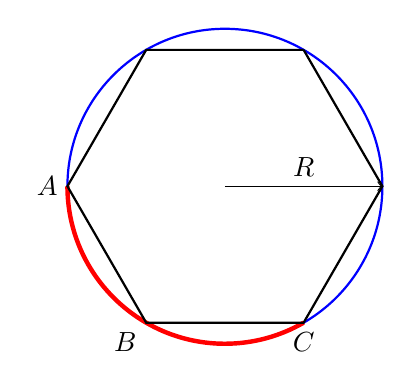
\begin{tikzpicture}
            \pgfmathsetmacro{\R}{2}
            \coordinate (O) at (0, 0);
            \coordinate (M) at ({\R/2*cos(60*6)}, {\R/2*sin(60*6)});
            
            \coordinate (P1) at ({\R*cos(60*1)}, {\R*sin(60*1)});
            \coordinate (P2) at ({\R*cos(60*2)}, {\R*sin(60*2)});
            \coordinate (P3) at ({\R*cos(60*3)}, {\R*sin(60*3)});
            \coordinate (P4) at ({\R*cos(60*4)}, {\R*sin(60*4)});
            \coordinate (P5) at ({\R*cos(60*5)}, {\R*sin(60*5)});
            \coordinate (P6) at ({\R*cos(60*6)}, {\R*sin(60*6)});

            \draw[thick, blue] (O) circle (\R);
            
            \node[anchor=east] at (P3) {$A$};
            \node[anchor=north east] at (P4) {$B$};
            \node[anchor=north] at (P5) {$C$};

            \draw[ultra thick, red] (P3) arc (180:300:\R);

            \draw[thick] (P1) -- (P2) -- (P3) -- (P4) -- (P5) -- (P6) -- (P1);

            \draw[->] (O) -- (P6);
            \node[anchor=south] at (M) {$R$};
        \end{tikzpicture}
    \end{center}

    Em um círculo, pode ser inscrito um hexágono regular
    com lados de comprimento $R$.
    
    A corda é determinada por dois pontos selecionados na circunferência.
    O primeiro ponto foi $B$.
    
    Para a corda ter comprimento menor do que o raio,
    o segundo ponto deve estar sobre o arco $\tikzarc{ABC}$,
    cujo comprimento é $\frac{1}{3}$ do comprimento da circunferência.

    A resposta é $1 - \frac{1}{3} = \frac{2}{3}$

    \begin{obs}
        Esta não é a única resposta para este problema,
        uma vez que há outras maneiras de selecionar uma corda
        ao acaso
    \end{obs}
\end{example}
